\section{Teclado N°. 1 - Mano izquierda}
    \label{chap:no1}

\subsection{Notas naturales abriendo}
\begin{center}
    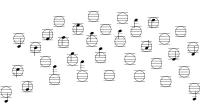
\includegraphics[width=0.8\textwidth]{./imgs/teclado_no1_iz_abrir}
\end{center}

\lilypondfile{./no1/iz_abrir.ly}
\hspace{0.1cm} \hline \hline

\subsection{Notas naturales cerrando}
\begin{center}
    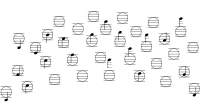
\includegraphics[width=0.8\textwidth]{./imgs/teclado_no1_iz_cerrar}
\end{center}

\lilypondfile{./no1/iz_cerrar.ly}
\hspace{0.1cm} \hline \hline

Este dibujo del teclado sirve para que el alumno puede estudiar la posición de
las notas naturales, sin el instrumento y con el instrumento.


\pagebreak
\section{Teclado N°. 1 - Mano derecha}

\subsection{Notas naturales abriendo}
\begin{center}
    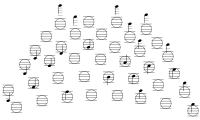
\includegraphics[width=0.8\textwidth]{./imgs/teclado_no1_de_abrir}
\end{center}

\lilypondfile{./no1/de_abrir.ly}
\hspace{0.1cm} \hline \hline

\subsection{Notas naturales cerrando}
\begin{center}
    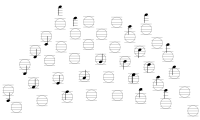
\includegraphics[width=0.8\textwidth]{./imgs/teclado_no1_de_cerrar}
\end{center}

\lilypondfile{./no1/de_cerrar.ly}
